\begin{activity} \label{A:3.1.3}  As pictured in the applet at~\href{http://gvsu.edu/s/9q}{\texttt{http://gvsu.edu/s/9q}}, a skateboarder who is $6$ feet tall rides under a $15$ foot tall lamppost at a constant rate of $3$ feet per second.  We are interested in understanding how fast his shadow is changing at various points in time.
\ba
	\item Draw an appropriate right triangle that represents a snapshot in time of the skateboarder, lamppost, and his shadow.  Let $x$ denote the horizontal distance from the base of the lamppost to the skateboarder and $s$ represent the length of his shadow.  Label these quantities, as well as the skateboarder's height and the lamppost's height on the diagram.
	\item Observe that the skateboarder and the lamppost represent parallel line segments in the diagram, and thus similar triangles are present.  Use similar triangles to establish an equation that relates $x$ and $s$.
	\item Use your work in (b) to find an equation that relates $\frac{dx}{dt}$ and $\frac{ds}{dt}$.
	\item At what rate is the length of the skateboarder's shadow increasing at the instant the skateboarder is $8$ feet from the lamppost?
	\item As the skateboarder's distance from the lamppost increases, is his shadow's length increasing at an increasing rate, increasing at a decreasing rate, or increasing at a constant rate?
	\item Which is moving more rapidly:  the skateboarder or the tip of his shadow?  Explain, and justify your answer.
\ea
\end{activity}
\begin{smallhint}
\ba
	\item Note that the lengths of the legs of the right triangle will be $15$ for the vertical one and $x + s$ for the horizontal one.
	\item The small triangle formed by the skateboarder and his shadow, with legs $6$ and $s$ is similar to the large triangle that has the lamppost as one of its legs.
	\item Simplify the equation in (b) as much as possible before differentiating implicitly with respect to $t$.
	\item Find $\left. \frac{ds}{dt} \right|_{x=8}$.
	\item Does the equation that relates $\frac{dx}{dt}$ and $\frac{ds}{dt}$ involve $x$?  Is $\frac{dx}{dt}$ changing or constant?
	\item Let $y$ represent the location of the tip of the shadow, so that $y = x + s$.
\ea
\end{smallhint}
\begin{bighint}
\ba
	\item Note that the lengths of the legs of the overall right triangle will be $15$ for the vertical one and $x + s$ for the horizontal one, with a smaller right triangle with legs of length 6 and $s$.
	\item The small triangle formed by the skateboarder and his shadow, with legs $6$ and $s$ is similar to the large triangle that has legs of length $15$ and $x + s$.  Remember that the ratios of the lengths of legs of similar triangles must be equal.
	\item Simplify the equation in (b) as much as possible before differentiating implicitly with respect to $t$.
	\item Find $\left. \frac{ds}{dt} \right|_{x=8}$.  Your answer should not depend on the value of $x$.
	\item Does the equation that relates $\frac{dx}{dt}$ and $\frac{ds}{dt}$ involve $x$?  Is $\frac{dx}{dt}$ changing or constant?
	\item Let $y$ represent the location of the tip of the shadow, so that $y = x + s$.  Observe that you can then write $\frac{dy}{dt}$ in terms of $\frac{dx}{dt}$ and $\frac{ds}{dt}$.
\ea
\end{bighint}
\begin{activitySolution}
\ba
	\item The given information leads us to construct the following diagram:
	\begin{center}
	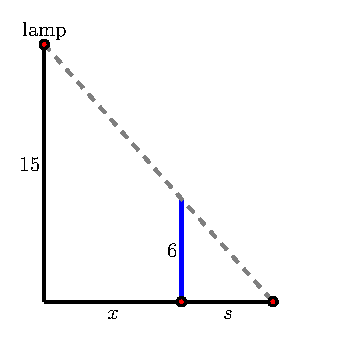
\includegraphics{figures/3_5_Act3Soln.eps}
	\end{center}
	\item The small triangle formed by the skateboarder and his shadow, with legs of length $6$ and $s$ is similar to the large triangle that has the lamppost as one of its legs (length 15) and horizontal leg of length $x + s$.  Because the ratios of the lengths of the legs of these two triangles is equal, we have
	$$\frac{s}{6} = \frac{s+x}{15}.$$  
	Simplifying, we have $15s = 6s + 6x$, so that $9s = 2x$, or most simply, $3s = 2x$.
	\item Differentiating with respect to $t$, it is immediate that $3 \frac{ds}{dt} = 2\frac{dx}{dt}$.
	\item Since $\frac{ds}{dt} = \frac{2}{3} \frac{dx}{dt}$, and $\frac{dx}{dt} = 3$, it follows $\frac{ds}{dt} = 2$ for every value of $t$ (and $x$).  Thus, $\left. \frac{ds}{dt} \right|_{x=8} = 2$ feet per second.
	\item Because $\frac{ds}{dt}$ is constant, the shadow's length is increasing at a constant rate (irrespective of the distance from the skateboarder to the lamppost). 
	\item Let $y$ represent the location of the tip of the shadow, so that $y = x + s$.  Observe that we can now compute $\frac{dy}{dt}$ in terms of $\frac{dx}{dt}$ and $\frac{ds}{dt}$, with $\frac{dy}{dt} = \frac{dx}{dt} + \frac{ds}{dt} = 3 + 2 = 5$ feet/sec, and hence the tip of the shadow is moving more rapidly than the skateboarder himself.
\ea
\end{activitySolution}
\aftera





